%Title of section
\section{基于动态伸缩的容器调度策略}

\subsection{系统结构}

\begin{frame}
\frametitle{系统结构}
\framesubtitle{调度系统模型}
\begin{block}{CaaS架构出现的问题}
\begin{itemize}
    \item 同一个应用对应多个容器副本
    \item 请求增加 $\Rightarrow$ \textbf{容器过载} $\Rightarrow$ 增加容器副本,分流请求,保证SLA
    \item 请求减小 $\Rightarrow$ \textbf{容器欠载} $\Rightarrow$ 减少容器副本,提升利用率,降低能耗
\end{itemize}
\end{block}
\begin{exampleblock}{解决方案:调度模型}
\begin{itemize}
    \item {\color{gray}预测容器负载,主动资源调整 $\Rightarrow$ \textbf{SAC-GPSO-SVM}}
    \item 负载预测结果与调整阈值 $\Rightarrow$ \textbf{容器扩容、缩容数量}
    \item 容器迁移、放置以及合并策略 $\Rightarrow$ \textbf{减少虚拟机和服务数量(已激活)}
\end{itemize}
\end{exampleblock}
\end{frame}

\begin{frame}
\frametitle{系统结构}
\framesubtitle{调度系统示意图}
\begin{figure}[htb]
    \centering
    \includegraphics[width=0.5\textwidth]{figures/fig14_scheduler_sys.jpg}
    \caption{基于动态伸缩的容器调度系统结构}
    \label{fig:fig14}
\end{figure}
\bigskip
\end{frame}

\subsection{问题定义}

\begin{frame}
\frametitle{问题定义}
\framesubtitle{CaaS架构容器能耗模型}
\begin{itemize}
    \item 数据中心在$t$时刻的能耗$P_{dc}(t)$(\textbf{仅考虑服务器})
    \begin{equation}
        P_{dc}(t) = \sum_{i=1}^{N_s} P_i(t)
    \end{equation}
    \item 服务器能耗$P_i(t)$,采用CPU能耗模型
    \begin{equation}
    \left\{
        \begin{array}{rcl}
            P_i(t) &=& a(t)F_p^i(U_i(t)) \\
            a(t) &\in& \{0,1\}
        \end{array}
    \right.
    \end{equation}
    \item 服务器CPU利用率$U_i(t)$主要受容器CPU利用率$U_c^{(k,j,i)}(t)$影响
    \begin{equation}
        U_i(t) = \sum_{j=1}^{N_{vm}}\sum_{k=1}^{N_c} U_c^{(k,j,i)}(t)
    \end{equation}
\end{itemize}
\end{frame}


\begin{frame}
\frametitle{问题定义}
\framesubtitle{调度目标}
\begin{itemize}
    \item 最小化CaaS数据中心总能耗
    \begin{equation}
    \begin{align*}
            &\min\quad P_{dc}(t)=\sum_{i=1}^{N_s} P_i(t)) \\
            &s.t.\quad
            \begin{cases}
            \sum_{j=1}^{N_{vm}}vm_{(j,i,r)}(t) < S_(i,r),\\
            \forall i \in [1,N_s],\ \forall r \in \{CPU,Memory,Disk,BW\} \\
            \\
            \sum_{k=1}^{N_{c}}c_{(k,j,i,r)}(t) < vm_(j,i,r),\\
            \forall i \in [1,N_{vm}],\ \forall r \in \{CPU,Memory,Disk,BW\}
            \end{cases}
    \end{align*}
    \end{equation}
\end{itemize}
\end{frame}

\begin{frame}
\frametitle{问题定义}
\framesubtitle{QoS指标}
\begin{itemize}
    \item SLA违反率:被分配的CPU资源小于请求的CPU资源量
    \begin{equation}
    \begin{align*}
        &SLA = \sum_{i=1}^{N_s}\sum_{j=1}^{N_{vm}}\sum_{p=1}^{N_v}
        \frac{CPU_r(vm_{ji},t_p) - CPU_a(vm_{ji},t_p)}{CPU_r(vm_{ji},t_p)} \\
        &\begin{cases}
            CPU_r(vm_{ji},t_p) = \sum_{k=1}^{N_c^{ji}}CPU_r(c_{kji},t_p) \\
            CPU_a(vm_{ji},t_p) = \sum_{k=1}^{N_c^{ji}}CPU_a(c_{kji},t_p)
        \end{cases}
    \end{align*}
    \end{equation}
    \item 容器对CPU资源的请求量:难以直接获取,需设定\textbf{超量因子(overbooking)}$P_n$
        \begin{enumerate}
            \item 从容器负载历史记录中选择一个负载值 $L_{per}$
            \item 概率 $P(L \le L_{per}) \ge P_n$
            \item $min(L_{per})$ 即为容器对CPU资源的请求量
        \end{enumerate}
\end{itemize}
\end{frame}

\subsection{调度算法}

\begin{frame}
\frametitle{调度算法}
\framesubtitle{负载检测与负载相关性分析}
\begin{itemize}
    \item 负载检测
    \begin{equation}
        Host\ status =
        \begin{cases}
            \textbf{Over-Load} \ \ \ if \ U_i(t) > T_{ol} \\
            \textbf{Under-Load} \ \ if\ U_i(t) < T_{ul}
        \end{cases}
    \end{equation}
    \item 负载相关性分析(皮尔森相关系数):\textbf{容器选择和主机选择算法}
    \begin{itemize}
        \item 容器负载历史记录:$X = {x_1,\cdots,x_n}$
        \item 主机负载历史记录:$Y = {y_1,\cdots,y_n}$
        \begin{equation}
            r_{xy} = \frac{\sum_{i=1}^n(x_i - \bar{x})(y_i - \bar{y})}
            {\sqrt{\sum_{i=1}^n(x_i - \bar{x})^2\sum_{i=1}^n(y_i - \bar{y})^2}}
        \end{equation}
    \end{itemize}
\end{itemize}
\end{frame}

\begin{frame}
\frametitle{调度算法}
\framesubtitle{容器伸缩算法}
\begin{itemize}
    \item 应用$V$当前的容器副本集:$\{v_1,\cdots,v_n\}$
    \item 容器副本负载区间上/下界的集合:$L^u = {l^u_1,\cdots,l^u_n}$ 和 $L^l = {l^l_1,\cdots,l^l_n}$
    \item 令应用$V$的副本总数$n=n_{now}$,则应用总体负载上下界:$L_v^u = \sum_{i=1}^{n_{now}}l_i^u$ 和 $L_v^l = \sum_{i=1}^{n_{now}}l_i^l$
    \item 设置应用$V$的总体负载阈值:
        \begin{itemize}
            \item 满足公式\ref{eq:lu} $\Rightarrow$ 扩容($L_v$离下界更近)
            \item 满足公式\ref{eq:ll} $\Rightarrow$ 缩容($L_v$离上界更近)
        \end{itemize}
    \begin{equation}
        \frac{L_v^u - n_{now} \times L_v}{n_{now} \times L_v - L^l_v} > 1
        \label{eq:lu}
    \end{equation}
    \begin{equation}
        \frac{(n_{now} - 1) \times L_v - L_v^l}{L_v^u - (n_{now} - 1) \times L_v} > 1
        \label{eq:ll}
    \end{equation}
\end{itemize}
\end{frame}

\begin{frame}
\frametitle{调度算法}
\framesubtitle{容器伸缩算法}
\begin{itemize}
    \item 满足扩容条件是的扩容数量:
    \begin{equation}
        \lceil \frac{(L_v^u+L_v^l)}{2L_v} - n_{now} \rceil
    \end{equation}
    \item 满足缩容条件是的缩容数量(至少保留一个副本):
    \begin{equation}
        \lceil n_{now} - \frac{(L_v^u+L_v^l)}{2L_v} {\color{red} - 1}\rceil
    \end{equation}
\end{itemize}
\end{frame}

\begin{frame}
\frametitle{调度算法}
\framesubtitle{容器选择算法 - 选择需迁移容器}
\begin{itemize}
    \item 从高负载主机列表($OLHL$)中选择需要迁移的容器:\textbf{负载高相关性}
\end{itemize}
\begin{algorithmic}[1]
  \Require{$OverLoadHostList(OLHL)$}
  \Ensure{$SelectedContainerList(SCL)$}
  \For{$host$ in $OLHL$}    \Comment{遍历高负载主机列表}
    \State $hostLoadHistory \gets host$.getLoadHistory() \Comment{主机负载记录}
    \State $containers \gets host$.getContainers()  \Comment{主机上的所有容器}
    \For{$container$ in $containers$} \Comment{计算容器与主机皮尔森系数}
      \State $containerLoadHistory \gets container$.getLoadHistory()
      \State $cor \gets$PearsonCor($containerLoadHistory $, $hostLoadHistory$)
      \State $cors$.put($container$, $cor$)
    \EndFor
    \State $cors$.sort(by=\textbf{cor}, order=\textbf{desc}) \Comment{相关度降序排列}
    \State $SCL$.add($cors$.first())    \Comment{添加相关度最高的容器}
  \EndFor \\
  \Return SCL
\end{algorithmic}
\bigskip
\end{frame}

\begin{frame}
\frametitle{调度算法}
\framesubtitle{容器选择算法 - 选择因缩容需删除的容器}
\begin{itemize}
    \item 从CPU利用率最低的开始删除:
    \begin{itemize}
        \item \textbf{大部分时间idle $\Rightarrow$ 额外资源浪费}
        \item \textbf{服务整体影响小 $\Rightarrow$ 延迟抖动小}
    \end{itemize}
\end{itemize}
\begin{algorithmic}[1]
  \Require{$ScaleDownContainerList(SDCL)$, $ScaleDownNumber(SDN)$}
  \Ensure{$SelectedContainerList(SCL)$}
  \For{$container$ in $SDCL$}   \Comment{遍历需要缩容的容器}
    \State $replicats \gets container$.getReplicats()   \Comment{获得这类容器所有副本}
    \State $replicats$.sort(by=\textbf{CPU}, order=\textbf{asc})    \Comment{CPU利用率升序排列}
    \State $sdn \gets$ get for this container from $SDN$    \Comment{获取缩容数量}
    \State $SCL$.add($replicats[0:sdn]$)    \Comment{选择该类容器前$sdn$个副本}
    \State $SDCL$.remove(replicats) \Comment{从列表中删除这类容器}
  \EndFor
  \State Send Container in $SCL$ to Remove
  \end{algorithmic}
\bigskip
\end{frame}

\begin{frame}[allowframebreaks]
\frametitle{调度算法}
\framesubtitle{容器迁移、放置和合并}
\begin{itemize}
    \item 主机选择算法(CorHS):为需要迁移、放置和合并的容器选择目的主机
\end{itemize}
\begin{algorithmic}[1]
   \Require{$AvailableHostList(AHL)$, $Container$, $Threshold(thr) 0<thr<1$}
   \Ensure{$Destination(Dest)$}
   \State $find \gets false$
   \State $containerLoadHistory \gets Container$.getLoadHistory()
   \While{$!find$}
     \For{$host$ in $AHL$}  \Comment{遍历候选主机}
     \State $hostLoadHistory \gets host$.getLoadHistory()\\
     \Comment{计算容器与候选主机负载相似度}
     \State $cor \gets$PearsonCor($containerLoadHistory $, $hostLoadHistory$)
     \If{$cor < thr$} \Comment{相似度低说明容器不会引起主机过载}
       \If{$host$.allocate($container$)}
         \State $Dest \gets (host, host$.getVm($container$)$)$
         \State $find \gets true$
         \State break
       \EndIf
     \EndIf
   \EndFor
   \State $thr \gets thr+0.1$ \Comment{找不到目的地,放松阈值条件}
   \If{$thr > 1$}
     \State $Dest \gets null$
   \EndIf
   \EndWhile \\
   \Return $Dest$
\end{algorithmic}
\end{frame}

\begin{frame}
\frametitle{调度算法}
\framesubtitle{容器迁移、放置和合并}
\begin{itemize}
    \item 容器迁移和放置:基于CorHS为迁移和放置容器选择目的地策略
\end{itemize}
\begin{algorithmic}[1]
  \Require{$OverloadHostList(OHL)$, $CML$, $ActiveHosts(AHs)$}
  \Ensure{$DestinationList(DL)$}
  \State $AvailableHostList(AHL) \gets AHs$.removeAll($OHL$)
  \State CML.sort(by=\textbf{CPU}, order=\textbf{desc}) \Comment{CPU降序排列待迁移容器列表}
  \For{$container$ in $CML$}    \Comment{遍历带迁移容器列表}
    \State $dest \gets$ CorHS($AHL$, $container$, \textbf{default} $thr$)   \Comment{CorHS算法选择目的地}
    \If{$dest \neq null$}   \Comment{目的地存在,添加迁移关系}
      \State $CML$.remove($container$)
      \State $DL$.add(($container$, $dest$))
    \Else   \Comment{目的地不存在,需要创建新虚拟机}
      \State \textbf{Send} $container$ to \textbf{VM Creator}
    \EndIf
  \EndFor\\
  \Return $DL$
  \end{algorithmic}
\end{frame}

\begin{frame}[allowframebreaks]
\frametitle{调度算法}
\framesubtitle{容器迁移、放置和合并}
\begin{itemize}
    \item 容器合并:基于CorHS将欠载主机上的容器进行合并的策略
\end{itemize}
\begin{algorithmic}[1]
  \Require
     $DestinationList(DL)$,
     $UnderloadHostList(UHL)$, $ActiveHosts(AHs)$
  \Ensure{$ContainersToMigrate(CTM)$}   \Comment{所有需要迁移或合并的容器}
  \State $AvailableHostList(AHL) \gets AHs$.removeAll(hosts in $DL$)
  \State $CTM$.addAll($DL$) \Comment{先添加因过载迁移需要迁移容器}
  \State $UHL$.sort(by=\textbf{CPU}, order=\textbf{asc})
  \For{$host$ in $UHL$} \Comment{遍历欠载主机}
    \If{$host$ is in $DL$}  \Comment{如果主机在过载迁移目的地中(\textbf{DL})}
      \State \textbf{continue}
    \Else
      \State $AHL$.remove($host$)   \Comment{暂时从$AHL$移除该主机}
      \State $containers \gets host$.getContainers()
      \For{$container$ in $containers$} \Comment{为全部容器选择新目的地}
        \State $dest \gets$ CorHS($AHL$, $container$)
        \If{$dest \neq null$}   \Comment{将迁移关系添加到临时列表}
          \State $containers$.remove($container$)
          \State $tempDestList$.add(($container$, $dest$))
        \EndIf
      \EndFor
      \If{$containers$.size() is equal to $0$}  \Comment{容器都可以被合并}
        \State $CTM$.addAll($tempDestList$) \Comment{$CTM$中加入需合并的容器}
        \State \textbf{Send} $host$ to \textbf{UL Host Deactivator} \Comment{请求关闭该主机}
      \Else
        \State $AHL$.add($host$) \Comment{将主机加回到$AHL$ \textbf{line 8}}
      \EndIf
    \EndIf
  \EndFor\\
  \Return $CTM$
  \end{algorithmic}
\end{frame}

\subsection{实验结果与分析}

\begin{frame}
\frametitle{实验结果与分析}
\framesubtitle{实验设置}
\begin{itemize}
    \item 容器负载数据(PlanetLab)、服务器和虚拟机配置、CloudSim
    \item 对比算法
    \begin{itemize}
        \item \textbf{FFHS(Kubernetes)}:选择第一台满足资源请求的主机
        \item \textbf{LFHS}:FFHS基础上增加主机CPU降序排列预处理
        \item \textbf{WEEC}:聚类划分容器,基于能耗特征的启发式算法
        \item \textbf{本文基于动态伸缩的容器调度策略}
    \end{itemize}
    \item 对照实验:
    \begin{itemize}
        \item 控制容器伸缩的\textbf{"应用总体负载阈值"$=70\%$}
        \item CorHS中的\textbf{"负载相关度阈值"$=0.5$}
    \end{itemize}
    \begin{table}[hftb]
        \centering
        \resizebox{0.8\textwidth}{!}{%
            \begin{tabular}{ccccc}
                \toprule
                \textbf{实验组} & \textbf{约束目标} & \textbf{UL} & \textbf{OL} & \textbf{Overbooking}\\
                \midrule
                group.1 & OL阈值 & $70\%$ & $[80\%,90\%,100\%]$ & $80th$\\
                group.2 & UL阈值 & $[50\%,60\%,70\%]$ & $80\%$ & $80th$ \\
                group.3 & Overbooking阈值& $70\%$ & $80\%$ & $[20th,40th,80th]$\\
                \bottomrule
            \end{tabular}
        }
        \caption{实验对照组设置}
        \label{tab:tab5}
    \end{table}
\end{itemize}
\end{frame}

\begin{frame}
\frametitle{实验结果与分析}
\framesubtitle{实验结果:group.1 \textbf{UL=$70\%$ OL=$[80\%,90\%,100\%]$, Overbooking=$80th$}}
\begin{minipage}{\textwidth}
    \centering
    \begin{figure}[htb]
    \centering
    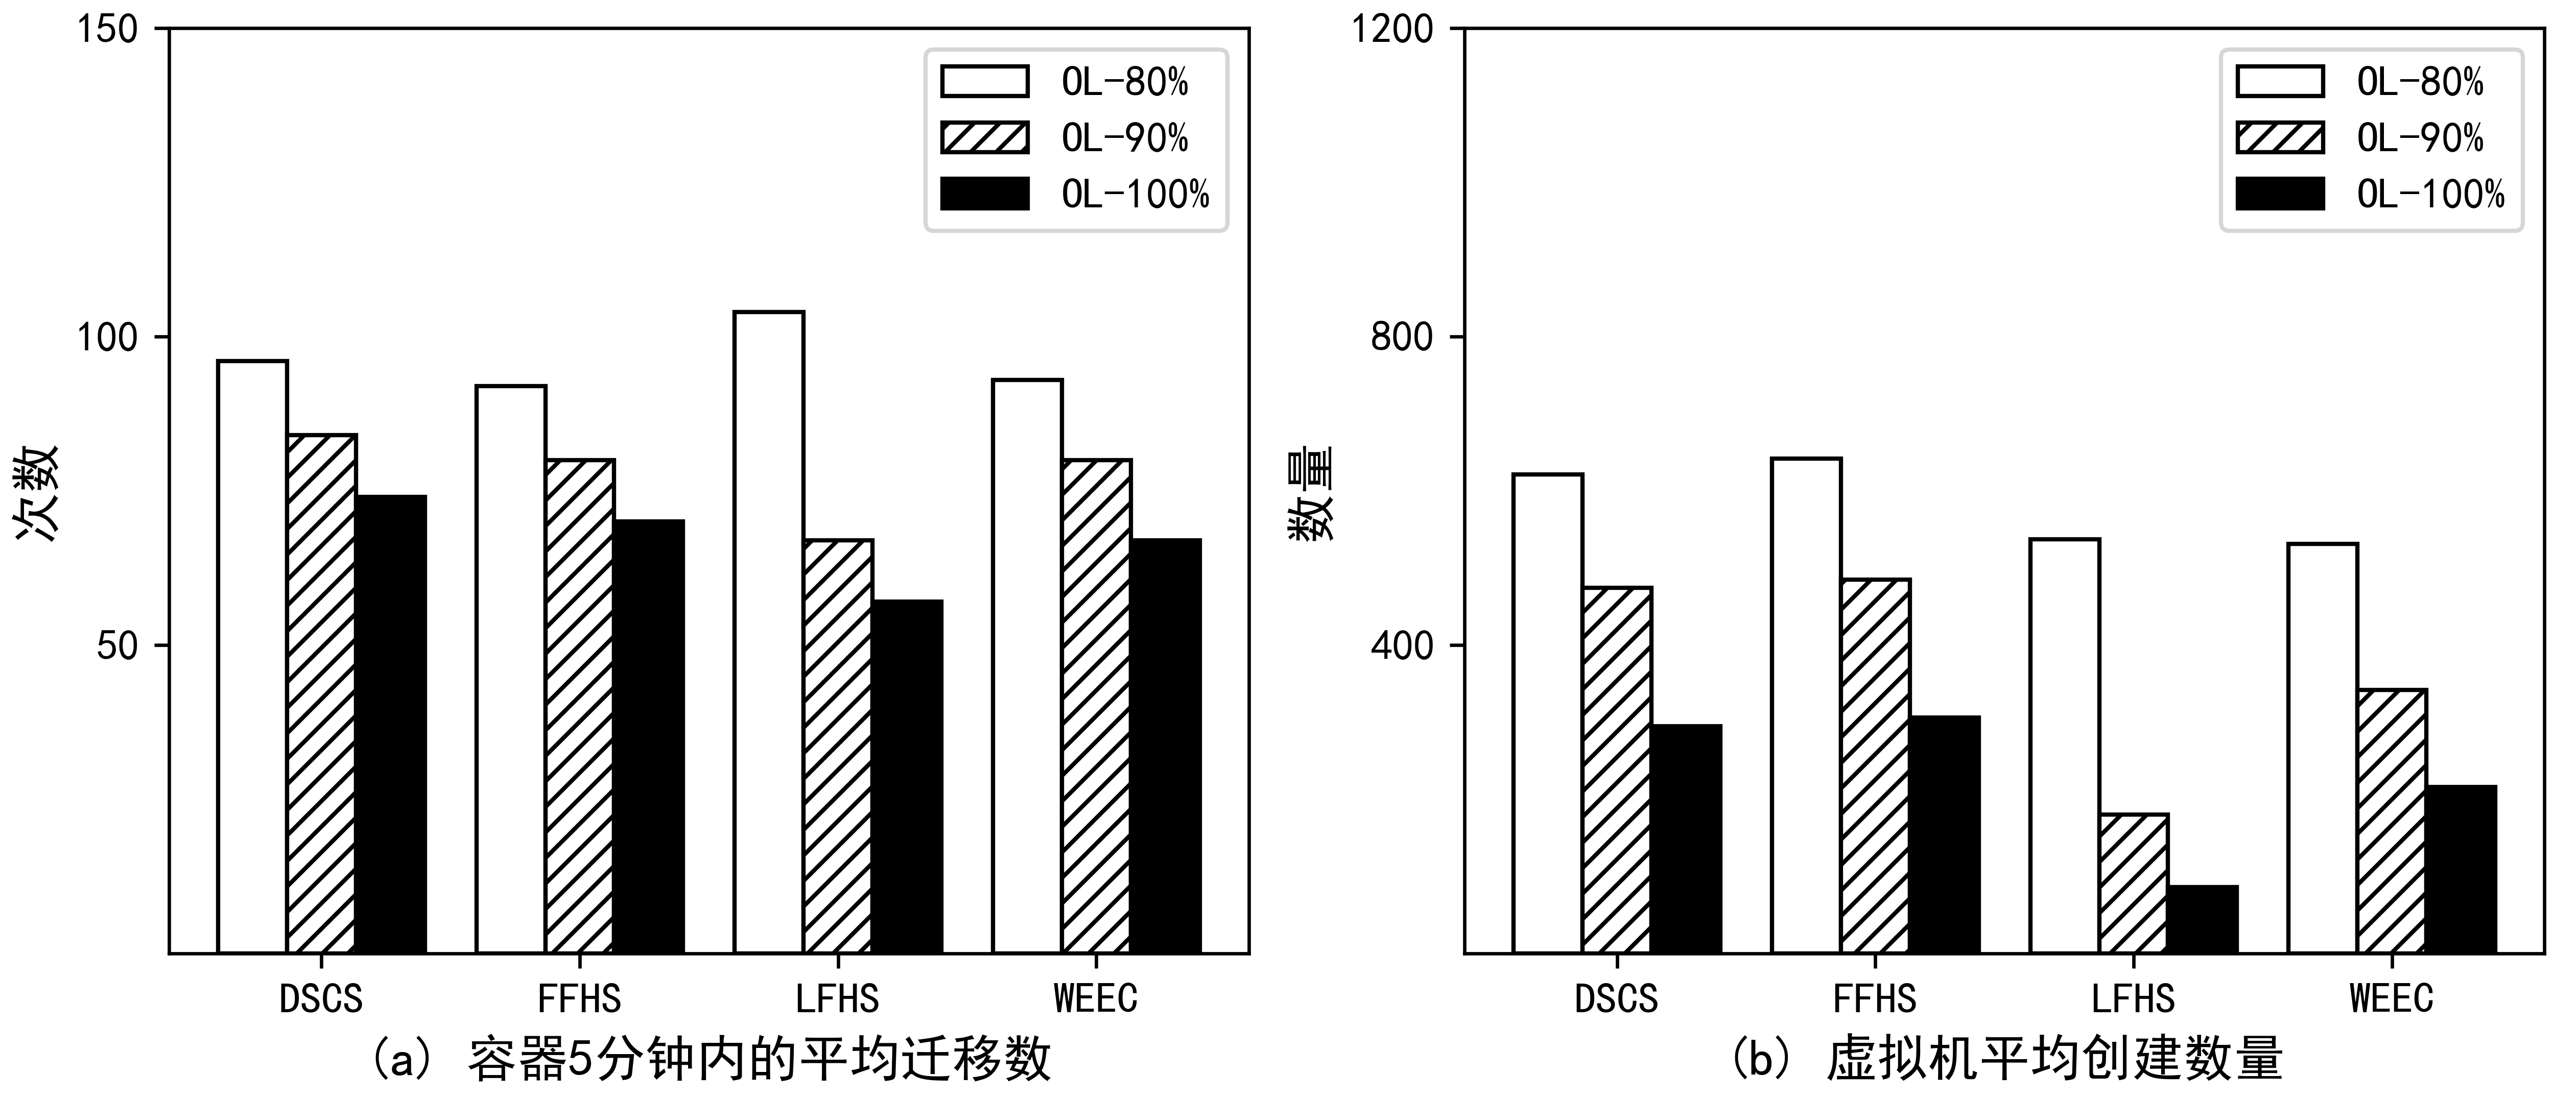
\includegraphics[width=0.45\textwidth]{figures/fig15_4-4_a.png}
    \end{figure}
\end{minipage}
\begin{minipage}{\textwidth}
    \centering
    \begin{figure}[htb]
    \centering
    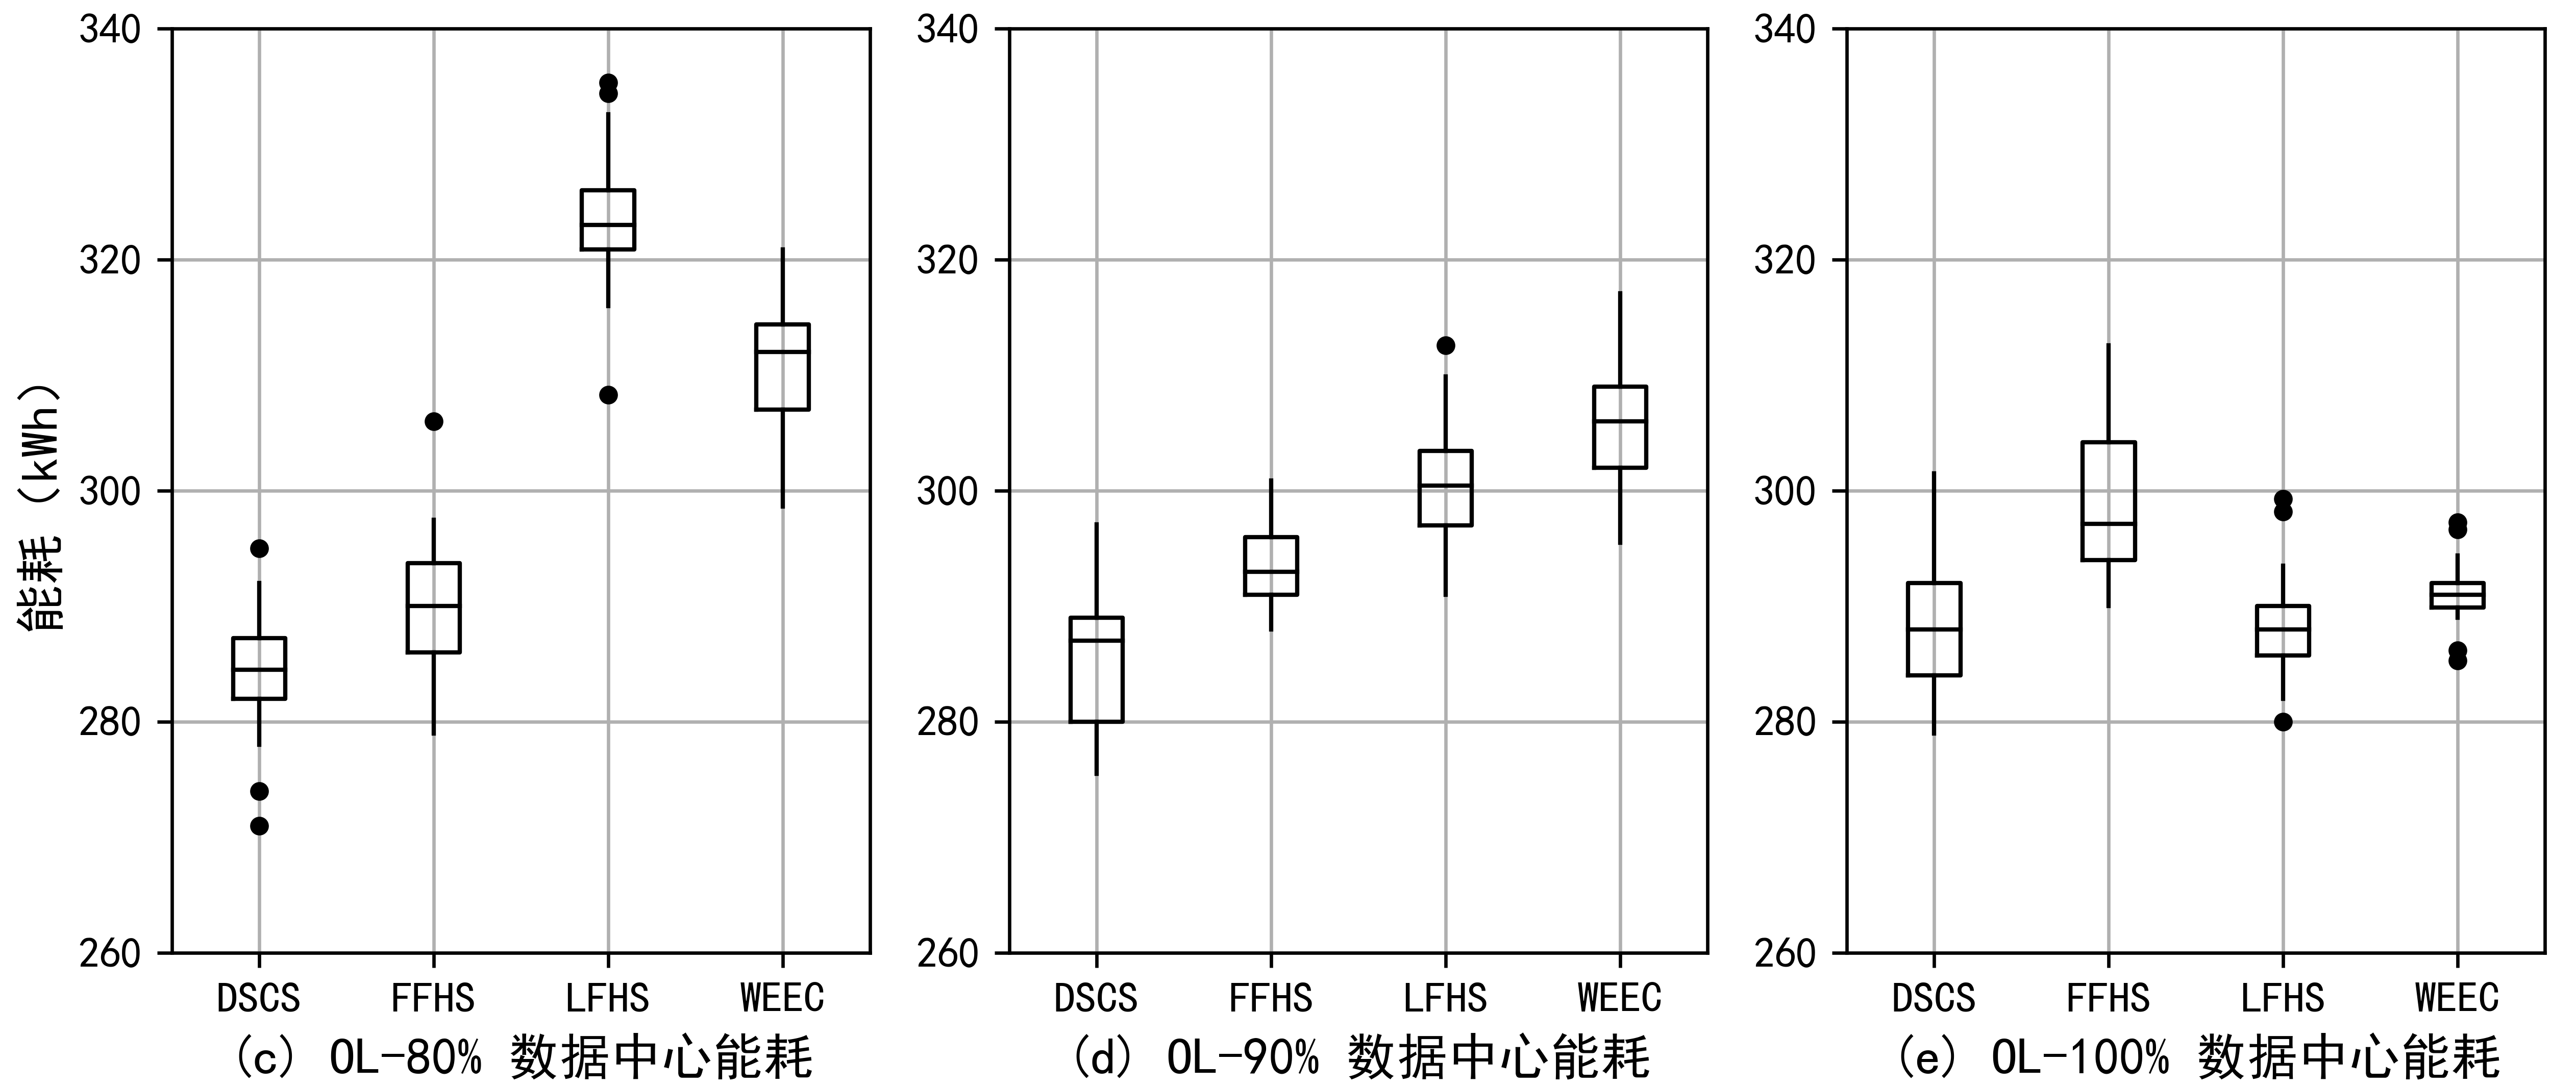
\includegraphics[width=0.45\textwidth]{figures/fig15_4-4_b.png}
    \end{figure}
\end{minipage}
\begin{minipage}{\textwidth}
    \centering
    \begin{figure}[htb]
    \centering
    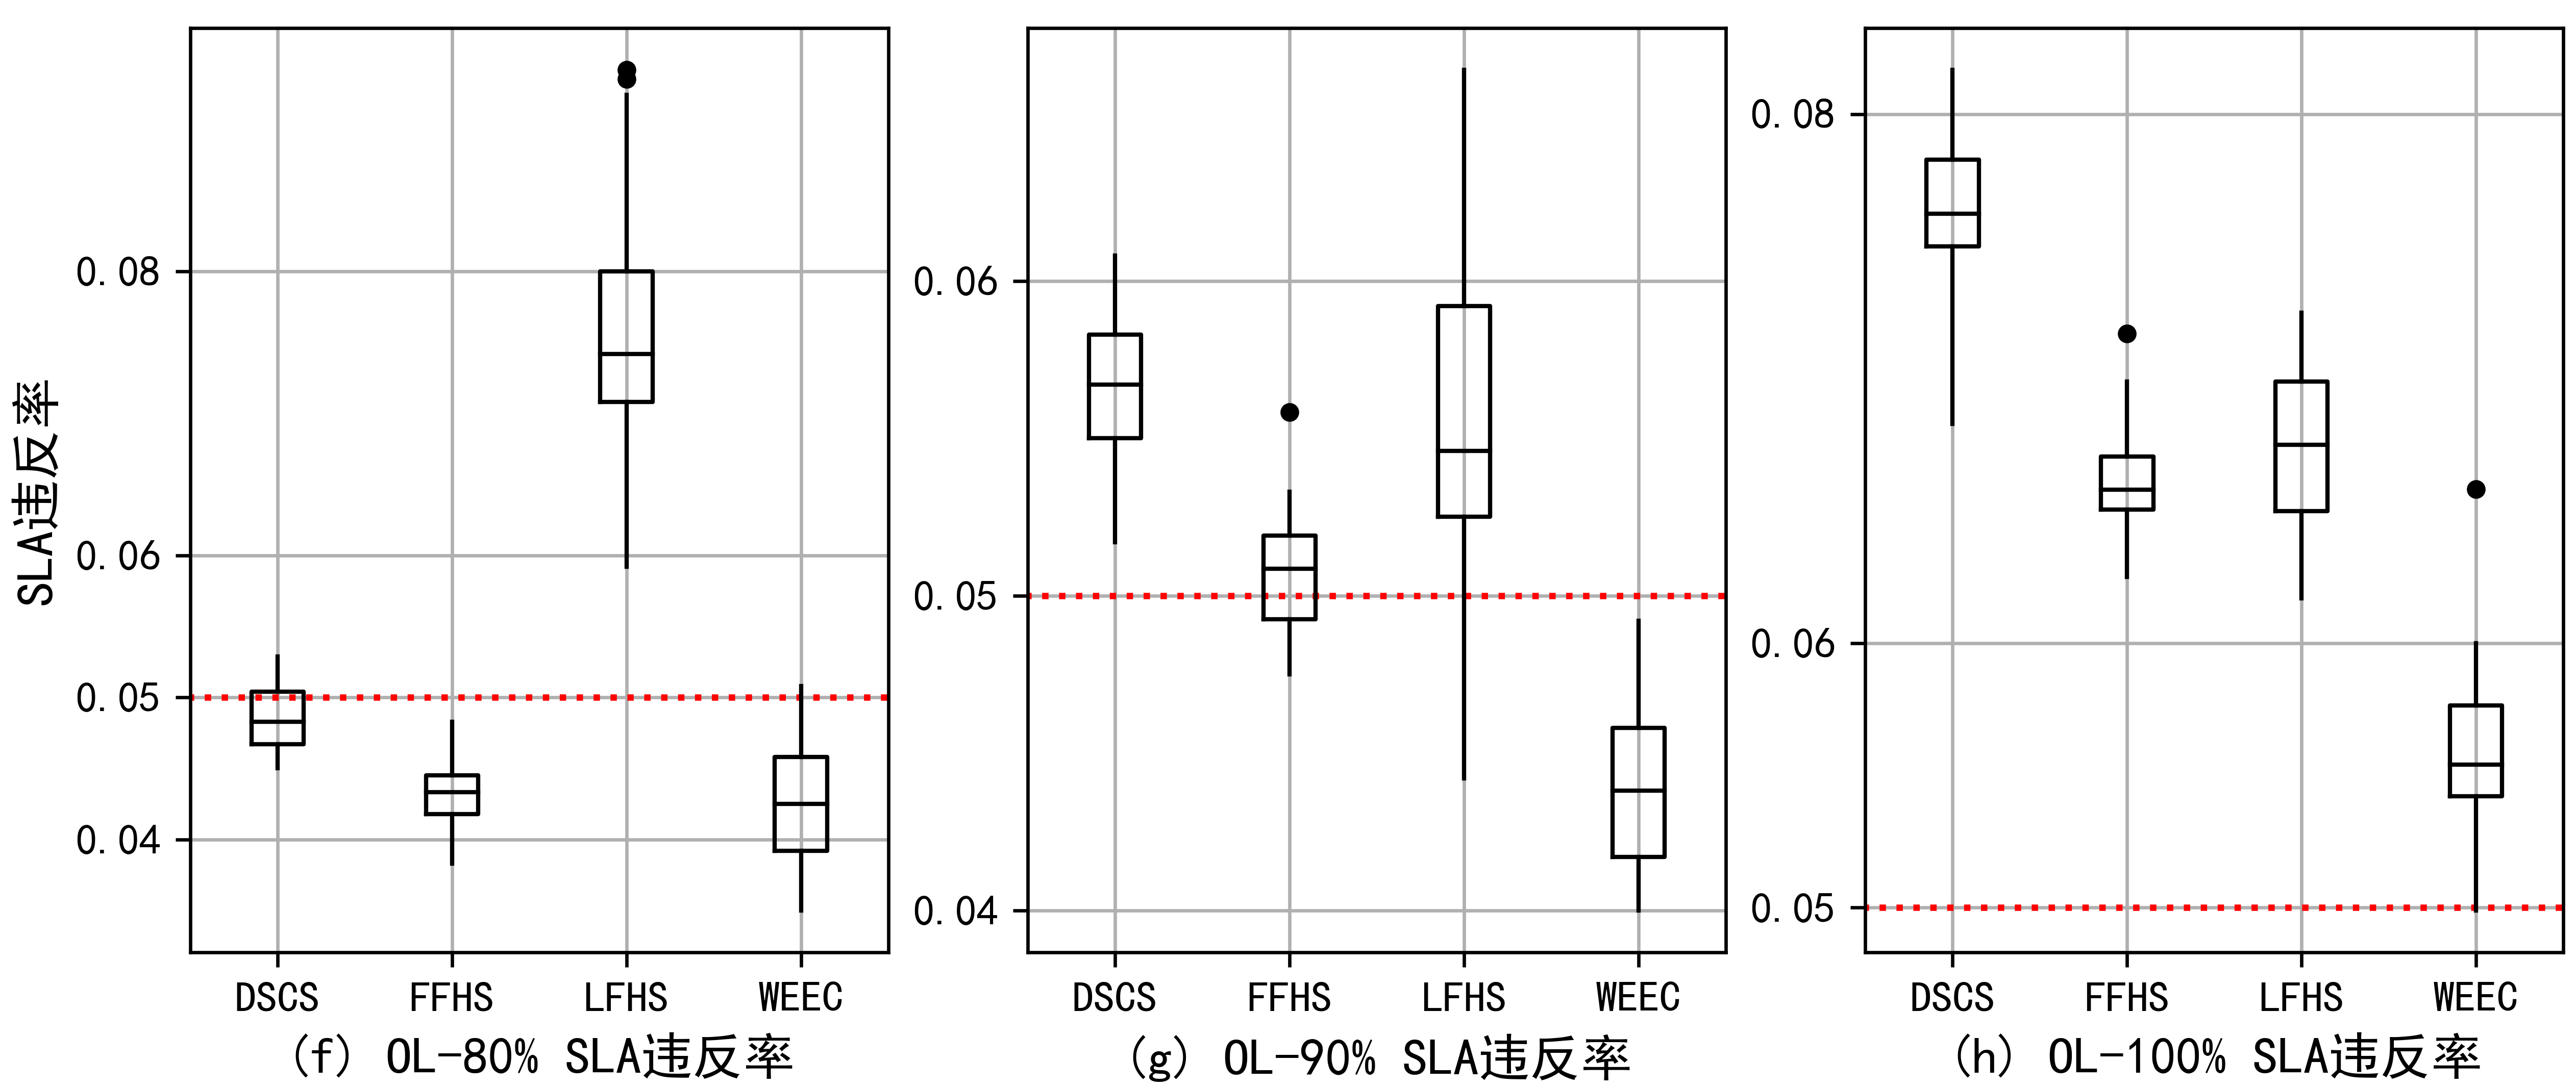
\includegraphics[width=0.45\textwidth]{figures/fig15_4-4_c.png}
    \caption{group.1 4种调度策略容器迁移、虚拟机创建数、能耗和SLA对比}
    \label{fig:fig15}
    \end{figure}
\end{minipage}
\end{frame}

\begin{frame}
\frametitle{实验结果与分析}
\framesubtitle{实验结果:group.2 \textbf{UL=$[50\%,60\%,70\%]$ OL=$80\%$, Overbooking=$80th$}}
\begin{minipage}{\textwidth}
    \centering
    \begin{figure}[htb]
    \centering
    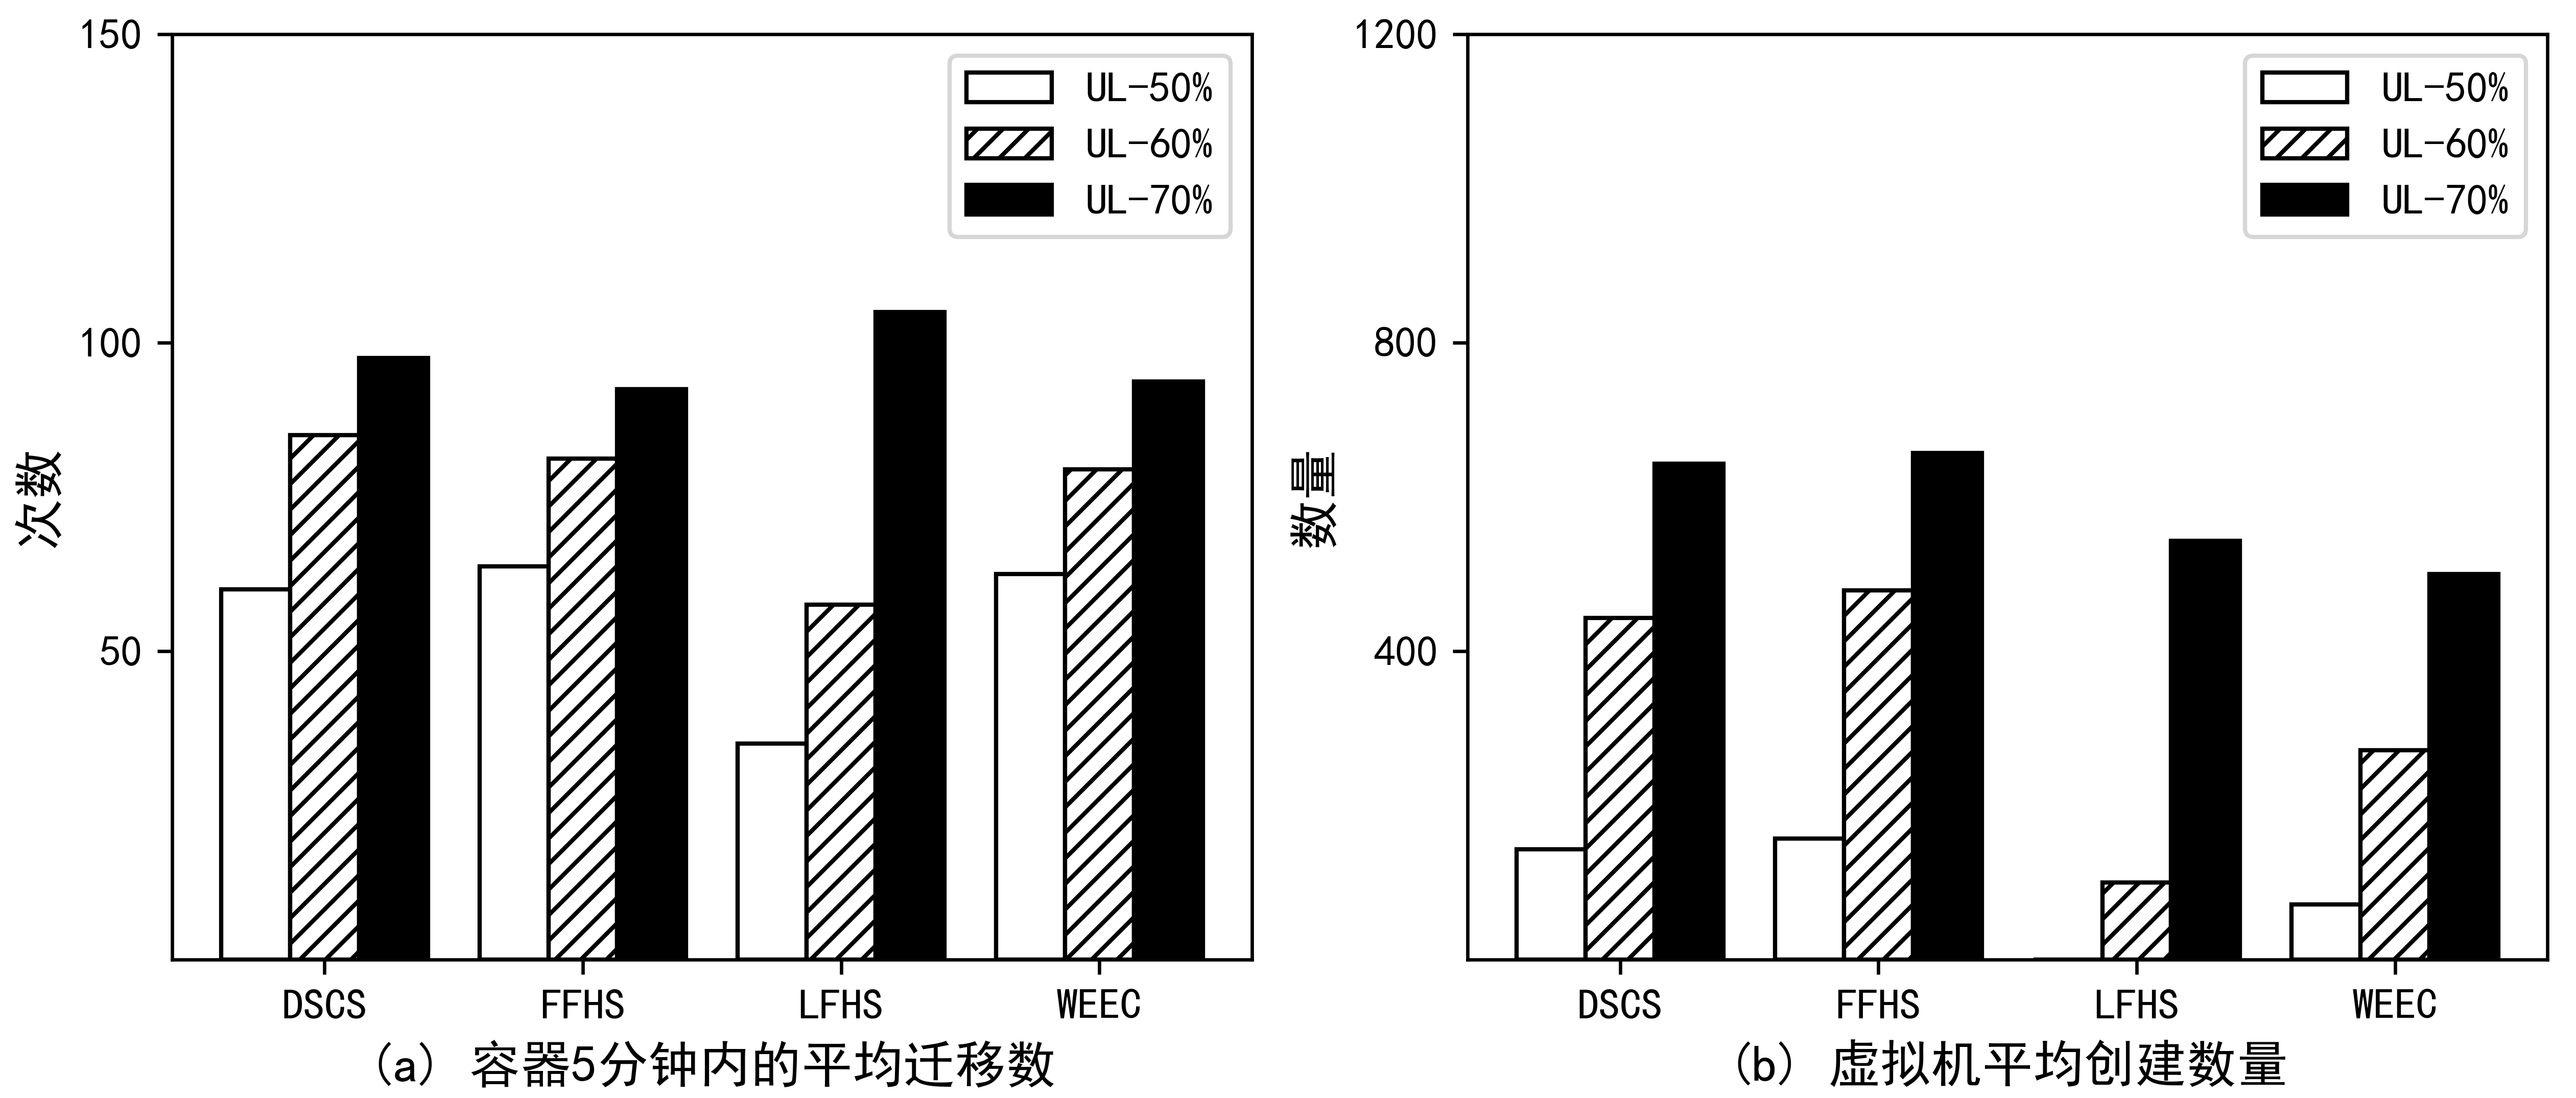
\includegraphics[width=0.45\textwidth]{figures/fig16_4-5_a.png}
    \end{figure}
\end{minipage}
\begin{minipage}{\textwidth}
    \centering
    \begin{figure}[htb]
    \centering
    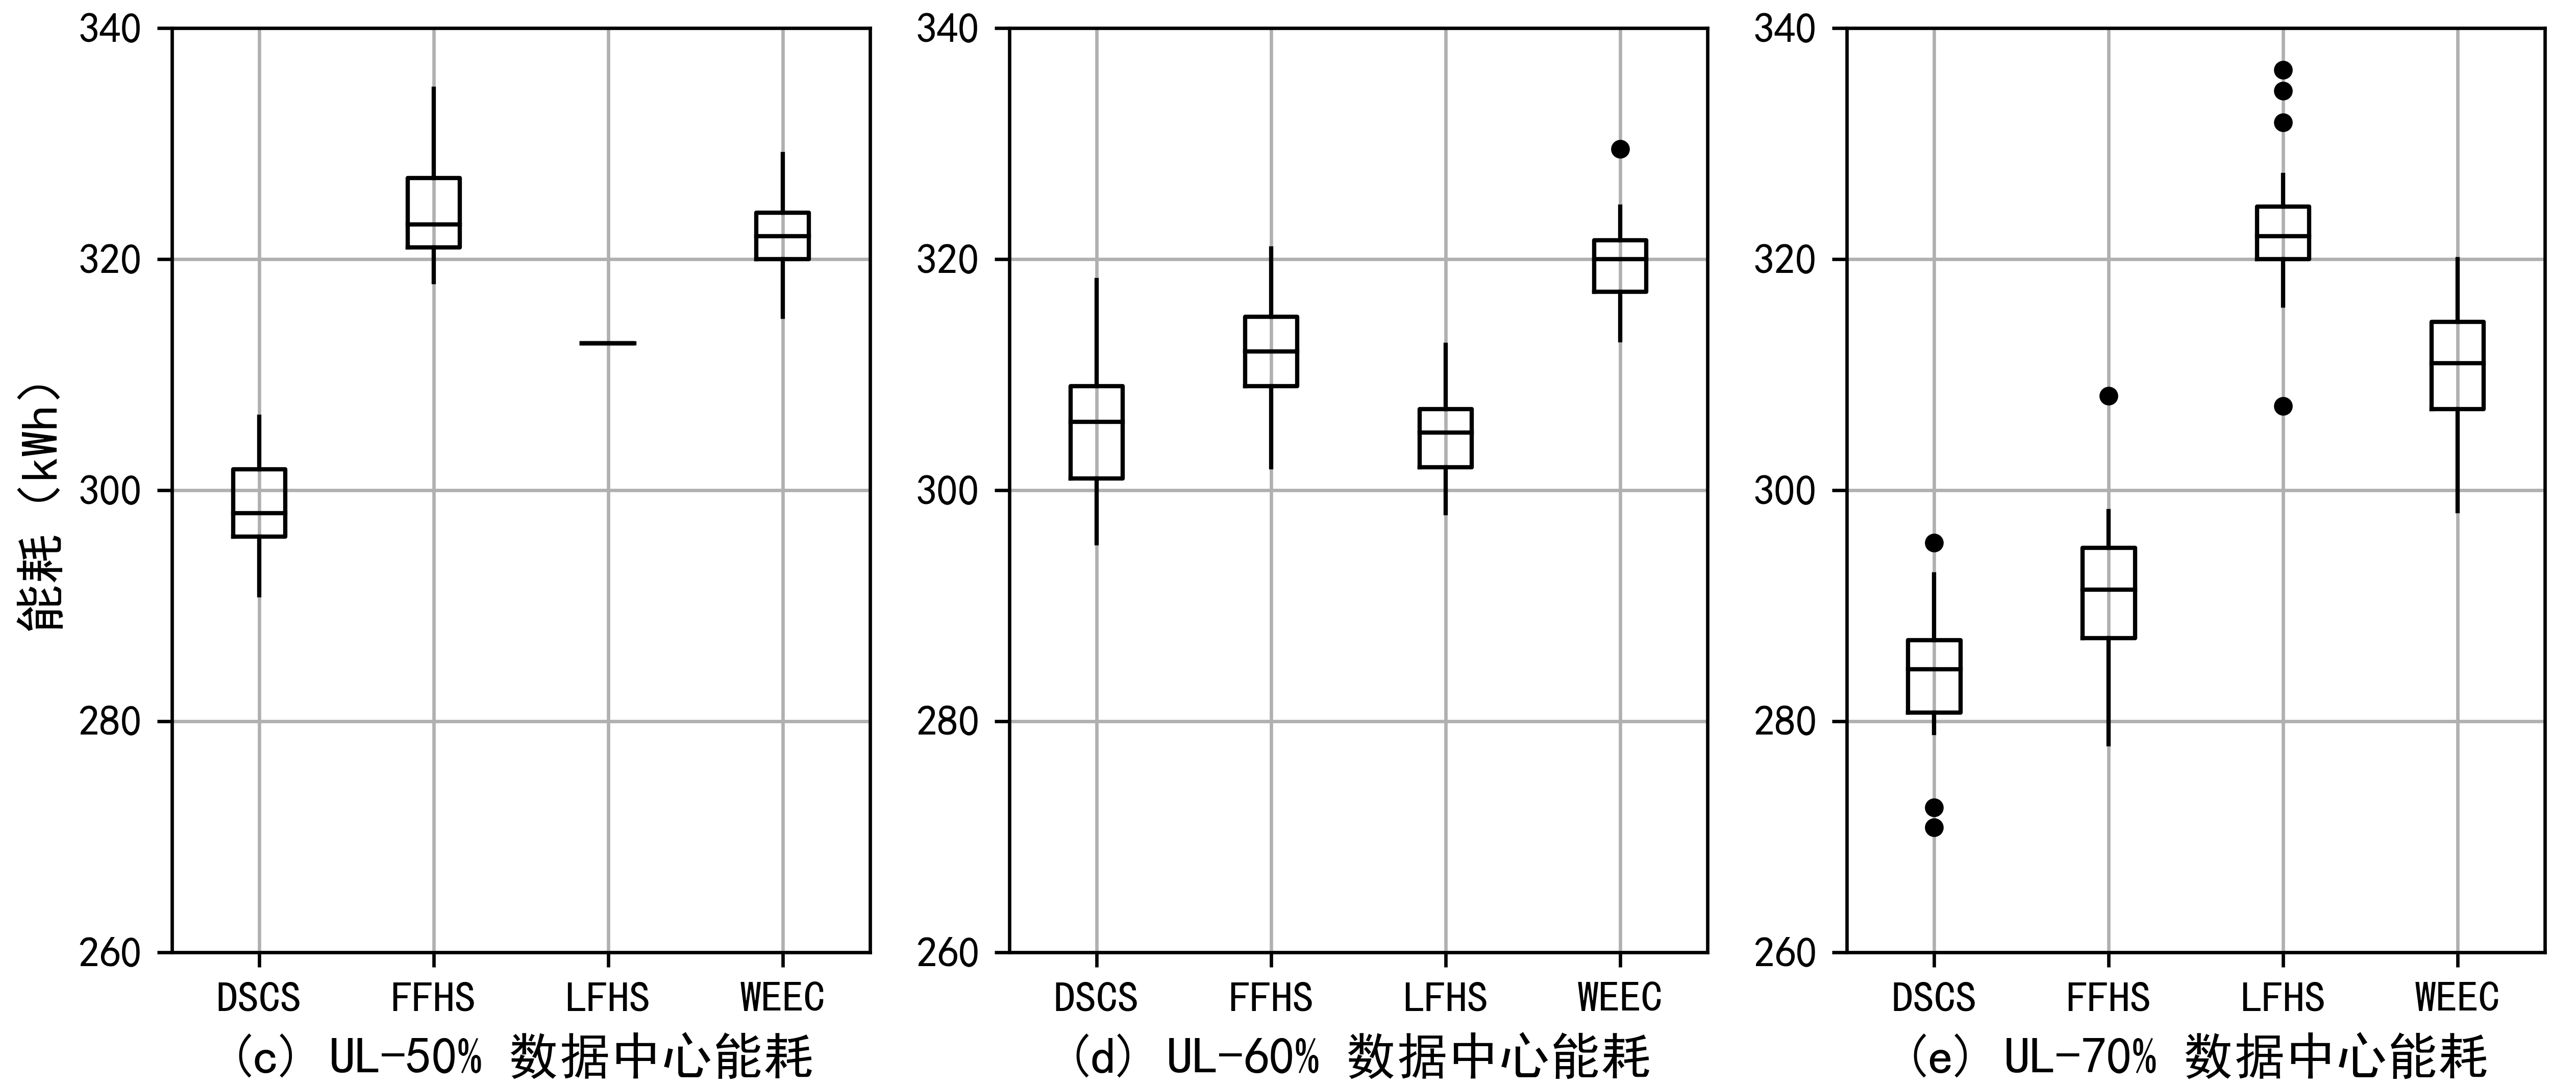
\includegraphics[width=0.45\textwidth]{figures/fig16_4-5_b.png}
    \end{figure}
\end{minipage}
\begin{minipage}{\textwidth}
    \centering
    \begin{figure}[htb]
    \centering
    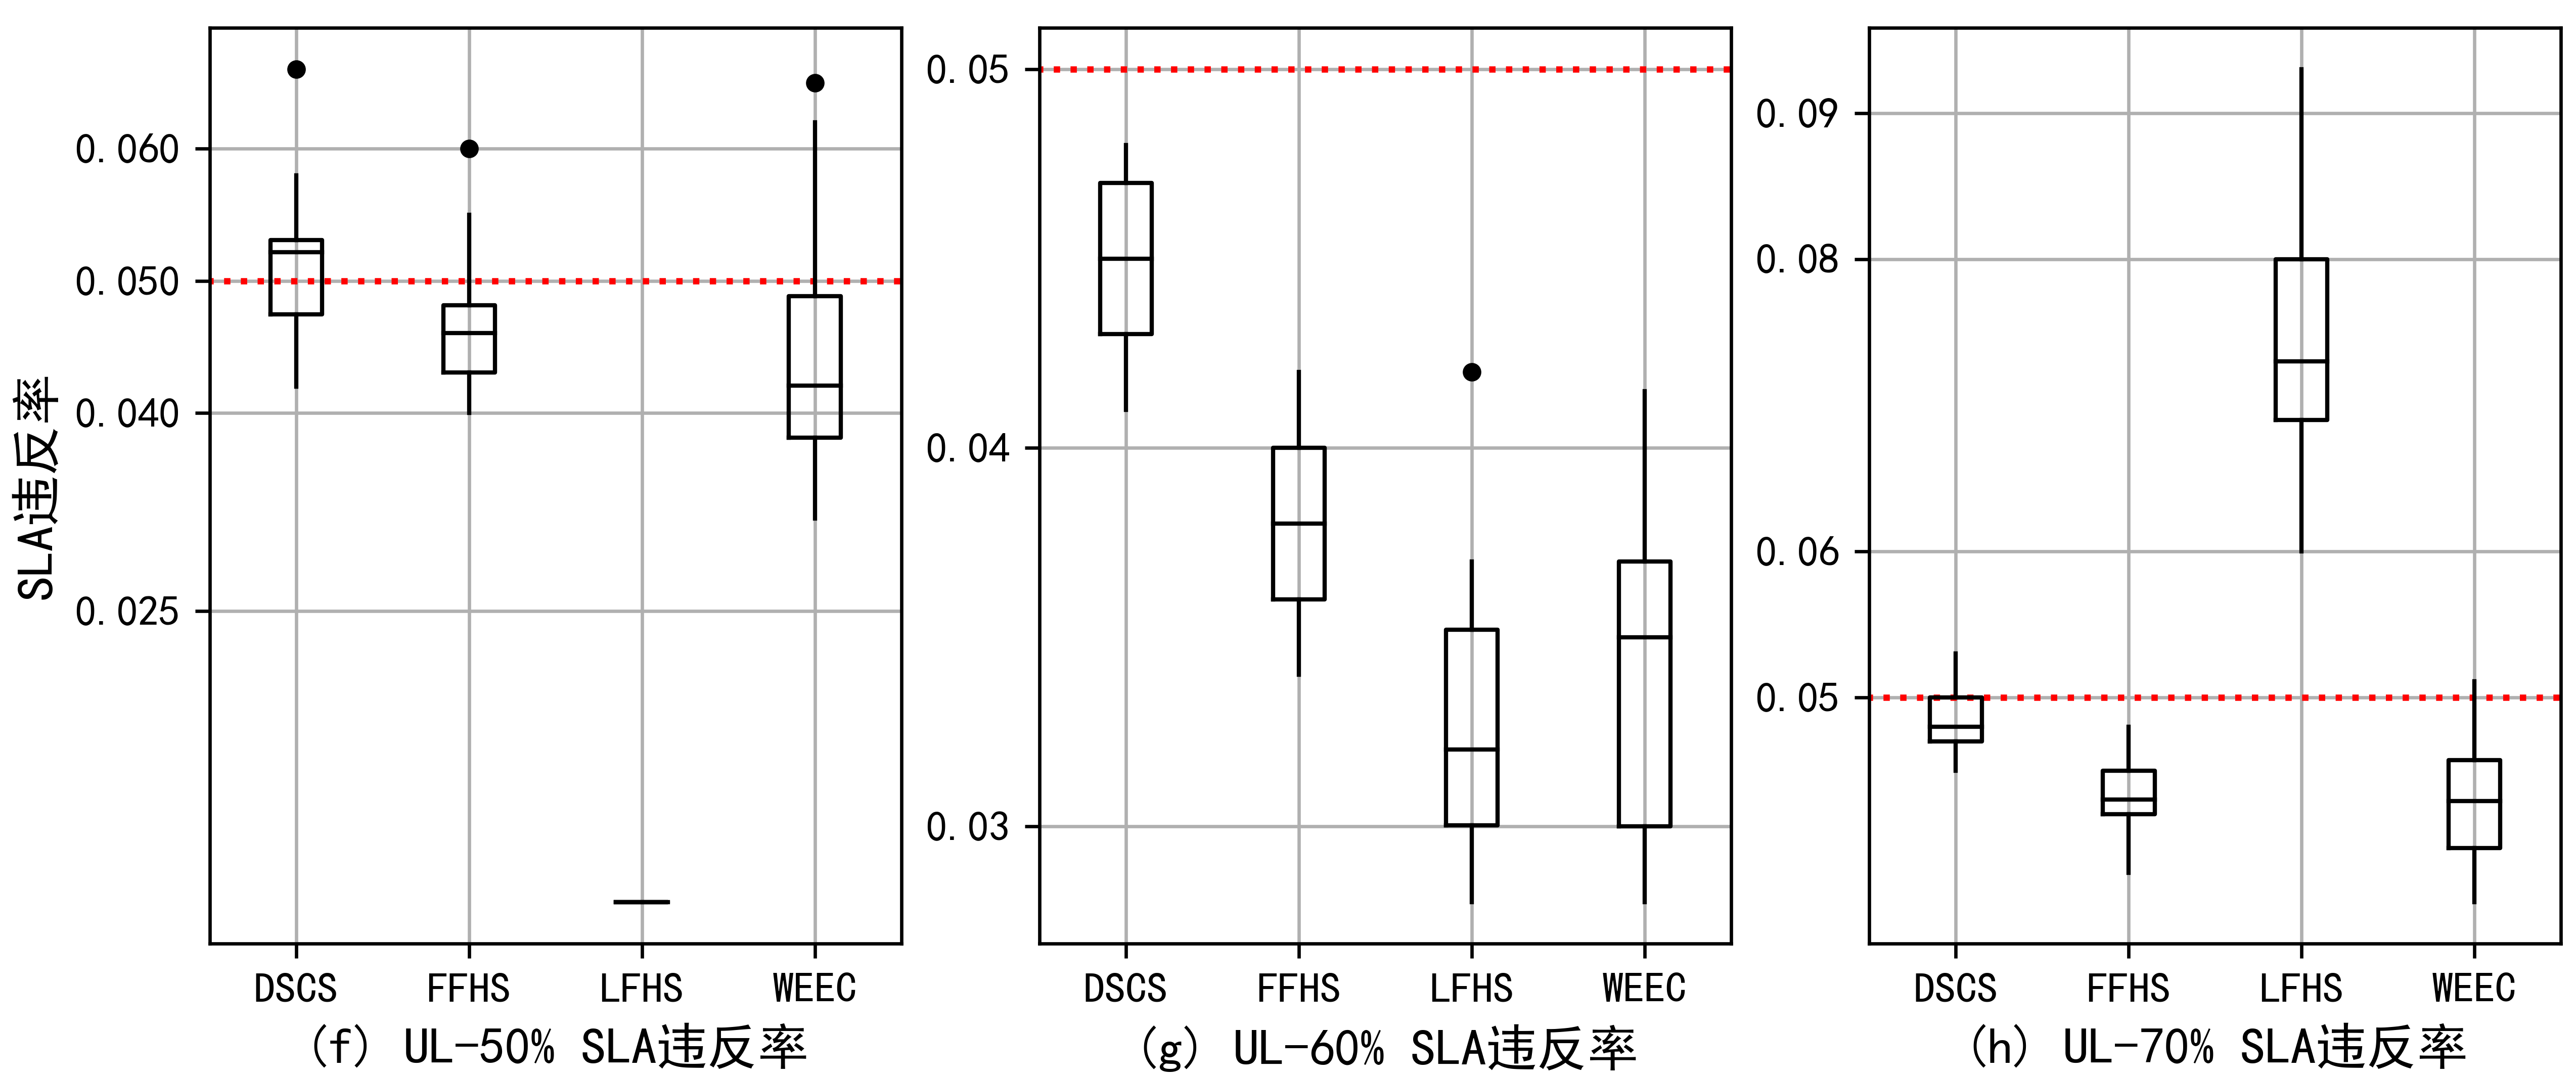
\includegraphics[width=0.45\textwidth]{figures/fig16_4-5_c.png}
    \caption{group.2 4种调度策略容器迁移、虚拟机创建数、能耗和SLA对比}
    \label{fig:fig16}
    \end{figure}
\end{minipage}
\end{frame}

\begin{frame}
\frametitle{实验结果与分析}
\framesubtitle{实验结果:group.3 \textbf{UL=$70\%$ OL=$80\%$, Overbooking=$[20th,40th,80th]$}}
\begin{minipage}{\textwidth}
    \centering
    \begin{figure}[htb]
    \centering
    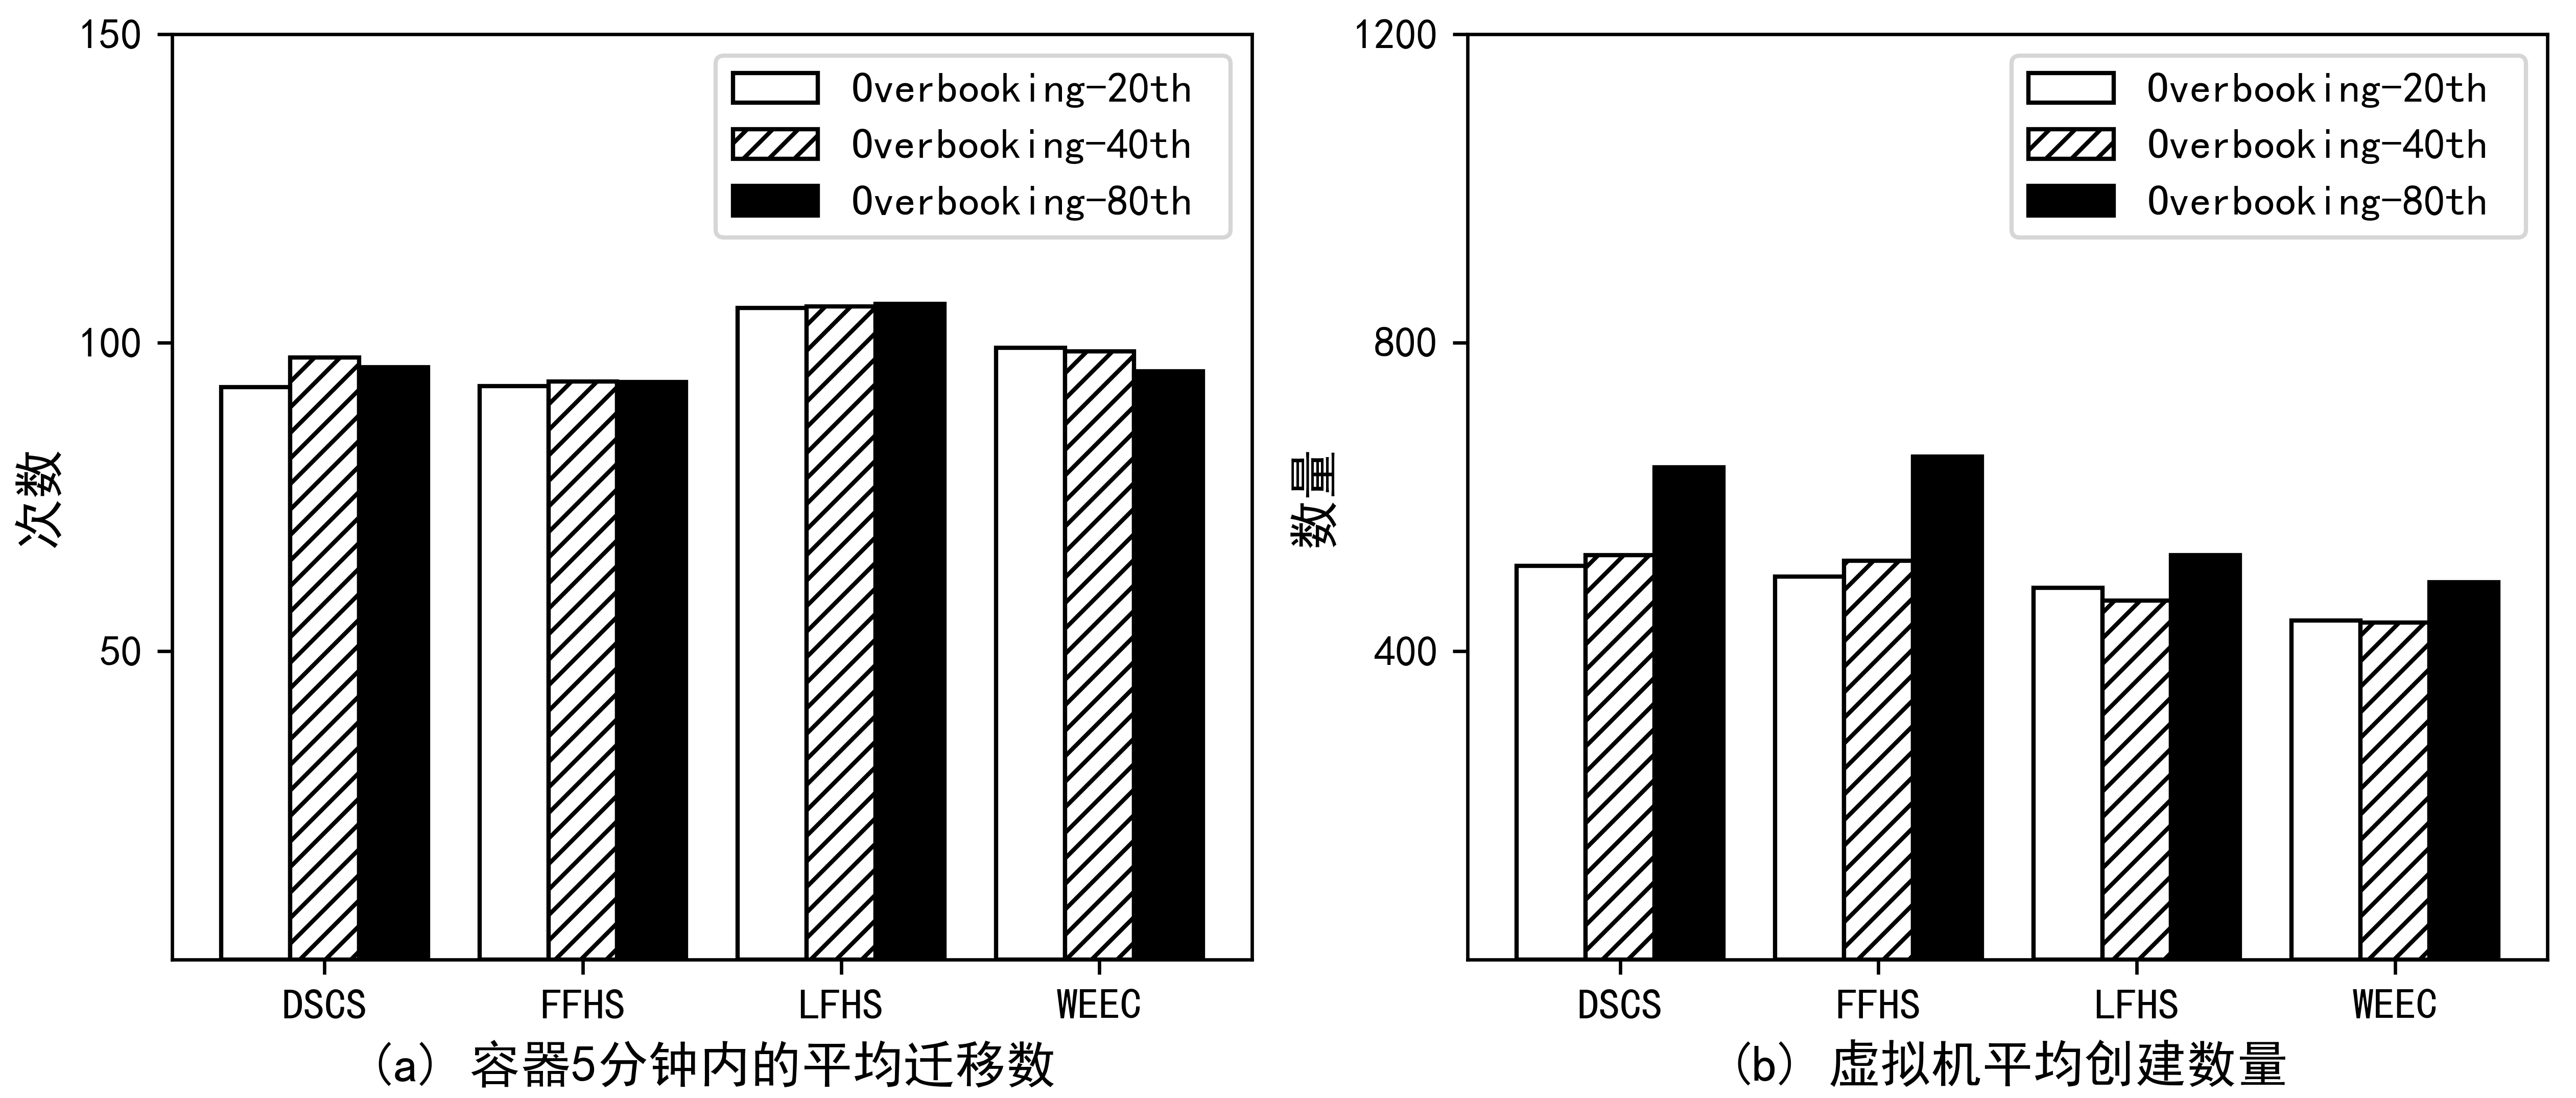
\includegraphics[width=0.45\textwidth]{figures/fig17_4-6_a.png}
    \end{figure}
\end{minipage}
\begin{minipage}{\textwidth}
    \centering
    \begin{figure}[htb]
    \centering
    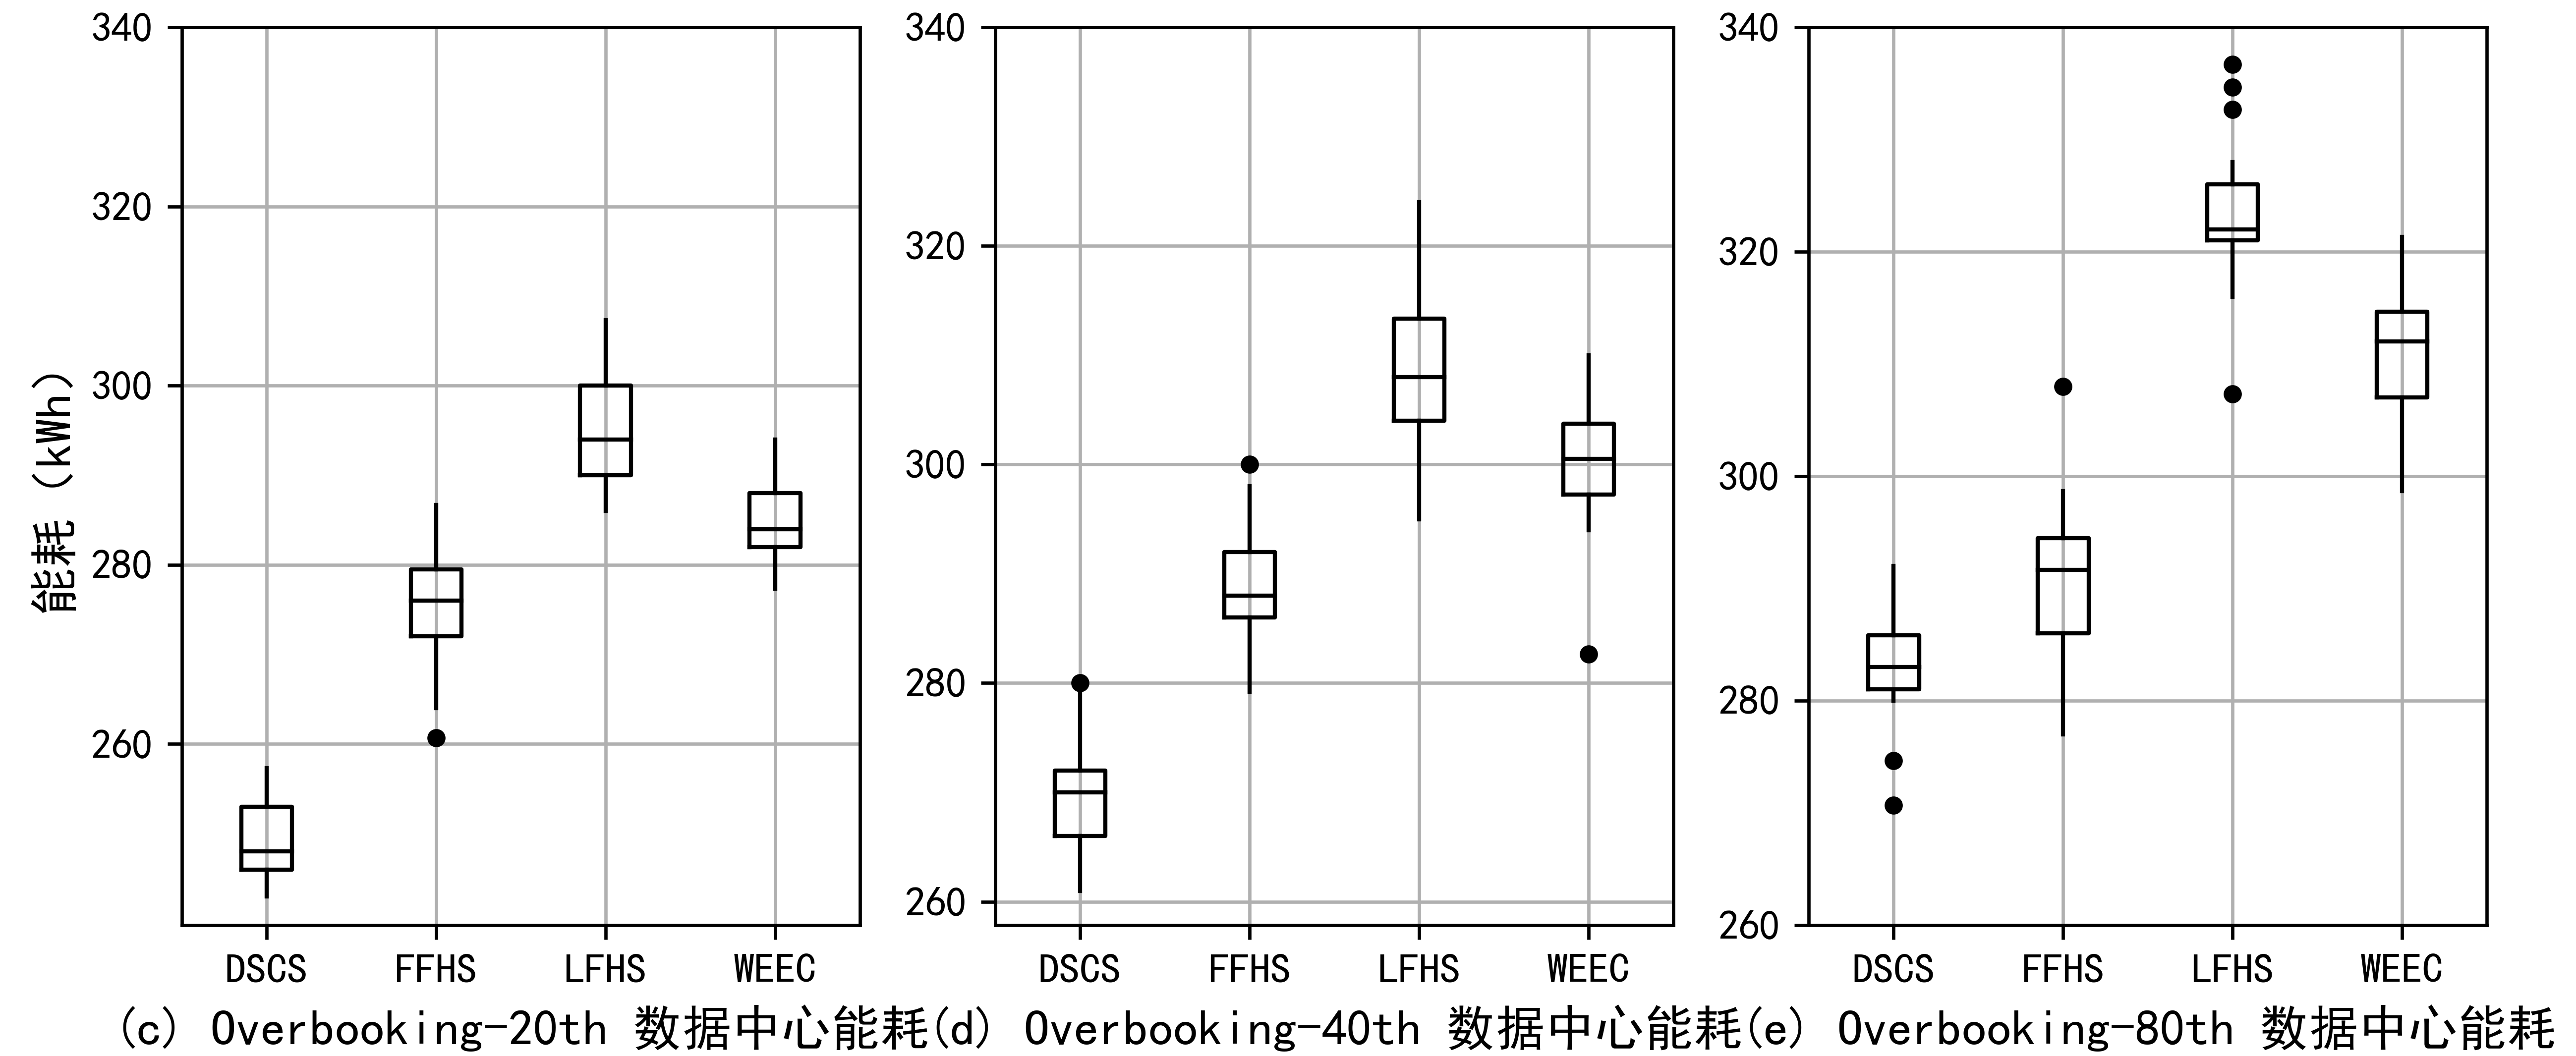
\includegraphics[width=0.45\textwidth]{figures/fig17_4-6_b.png}
    \end{figure}
\end{minipage}
\begin{minipage}{\textwidth}
    \centering
    \begin{figure}[htb]
    \centering
    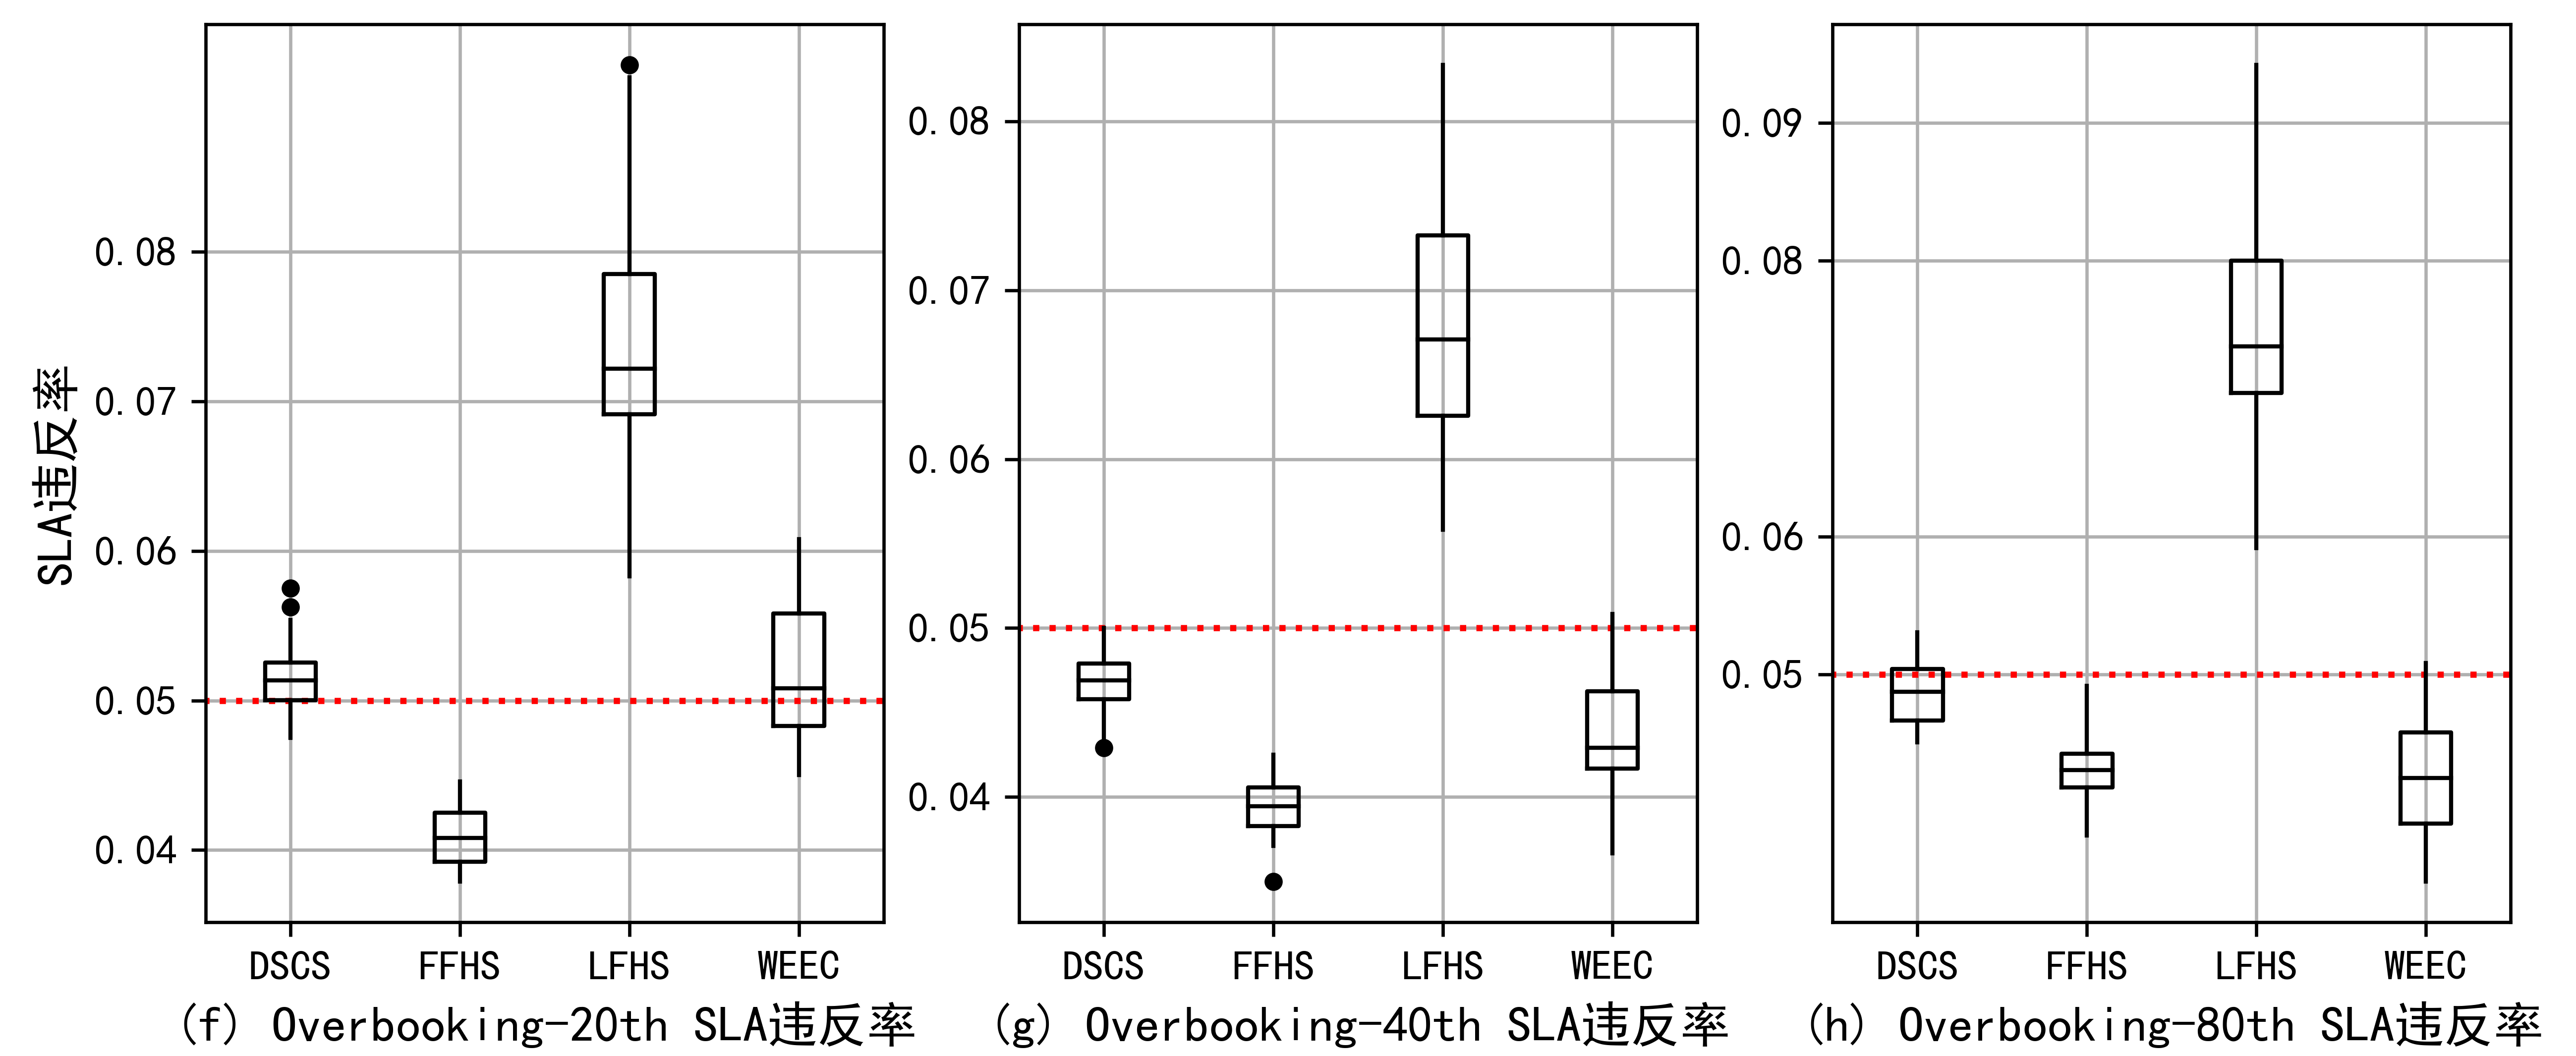
\includegraphics[width=0.45\textwidth]{figures/fig17_4-6_c.png}
    \caption{group.3 4种调度策略容器迁移、虚拟机创建数、能耗和SLA对比}
    \label{fig:fig17}
    \end{figure}
\end{minipage}
\end{frame}

\begin{frame}
\frametitle{实验结果与分析}
\framesubtitle{SLA违反补偿协议}
\begin{itemize}
    \item 主流云服务商(GCP\footnote{\tiny{https://cloud.google.com/}},
    AWS\footnote{\tiny{https://aws.amazon.com/}},阿里云\footnote{\tiny{https://cn.aliyun.com/}})SLA违反补偿协议
\end{itemize}
\begin{table}[hftb]
        \centering
        \resizebox{0.8\textwidth}{!}{%
            \begin{tabular}{ccccc}
                \toprule
                \textbf{赔偿(相对于租金比例)} & \textbf{SLA违反率(未响应时间占比)} \\
                \midrule
                $0$ & $0\sim5\%$   \\
                $5$ & $5\%\sim15\%$   \\
                $10$ & $15\%\sim20\%$   \\
                $20$ & $20\%\sim25\%$   \\
                $35$ & $25\%\sim30\%$   \\
                $55$ & $30\%\sim45\%$   \\
                $80$ & $45\%\sim50\%$   \\
                $100$ & $50\%$以上   \\
                \bottomrule
            \end{tabular}
        }
        \caption{主流云供应商SLA违反补偿金计算}
        \label{tab:tab6}
    \end{table}
\end{frame}